\Chapter{Tervezés}

A következőkben bemutatom a különböző szerepköröket és folyamatokat a szekvenciadiagramok és folyamatábrák segítségével. Részletes elemzésre kerülnek a lapok közötti átmenetek és az adatmodell is. Ezek a lépések nélkülözhetetlenek a hatékony és átlátható tervezéshez, hogy sikeresen elkészülhessen a projekt.

\Section{Szerepkörök leírása}

A webalkalmazás kialakítása során hat különböző szerepkört határoztam meg, amelyek mindegyike különös felelősséggel és jogosultságokkal rendelkezik a platformon. Ezek a szerepkörök a következők:

\begin{enumerate}
\item Hallgató
\begin{itemize}
\item Szakdolgozat létrehozása, szerkesztése és mentése a rendszerben.
\item Az elkészült dolgozat benyújtása a rendszeren keresztül.
\item Visszajelzések és észrevételek megtekintése a dolgozatról a bírálók, témavezető vagy a bizottság részéről.
\item A bírálók és a bizottság értékeléseinek megtekintése.
\item A védés időpontjának és helyszínének megtekintése és kezelése.
\item A végső értékelés és jegy megtekintése.
\end{itemize}

\item Bíráló
\begin{itemize}
\item A dolgozat értékelése és visszajelzés küldése a hallgatónak.
\item A dolgozat nyomon követése és annak státuszának frissítése a rendszerben.
\item Az értékelőlap és a végső jegy rögzítése a rendszerben.
\end{itemize}

\item Záróvizsga jegyzője
\begin{itemize}
\item A záróvizsga időpontjának és helyszínének meghatározása és frissítése.
\item A záróvizsga résztvevőinek (hallgató, bírálók, bizottság) értesítése és meghívók kiküldése.
\item A záróvizsga jegyzőkönyvének vezetése és rögzítése a rendszerben.
\end{itemize}

\newpage
\item Záróvizsga bizottság elnöke
\begin{itemize}
\item A bizottság tagjainak kijelölése és módosítása.

\item A záróvizsga menetének és a kérdéseknek meghatározása.

\item A hallgató szakdolgozatának értékelése a bizottság véleménye alapján.

\item A végső értékelés rögzítése a rendszerben.
\end{itemize}

\item Témavezető

\begin{itemize}
\item A hallgatóval való kommunikáció és támogatás a szakdolgozat elkészítése során.

\item A hallgató dolgozatának nyomon követése és visszajelzések küldése.

\item A bírálók és a bizottság értékeléseinek megtekintése.

\item A végső értékelés és jegy rögzítése a rendszerben.


\end{itemize}

\item Adminisztrátor

\begin{itemize}

\item Az adminisztrátor a fentiek mindegyikével rendelkezik.

\end{itemize}

\end{enumerate}

\begin{figure}[ht]
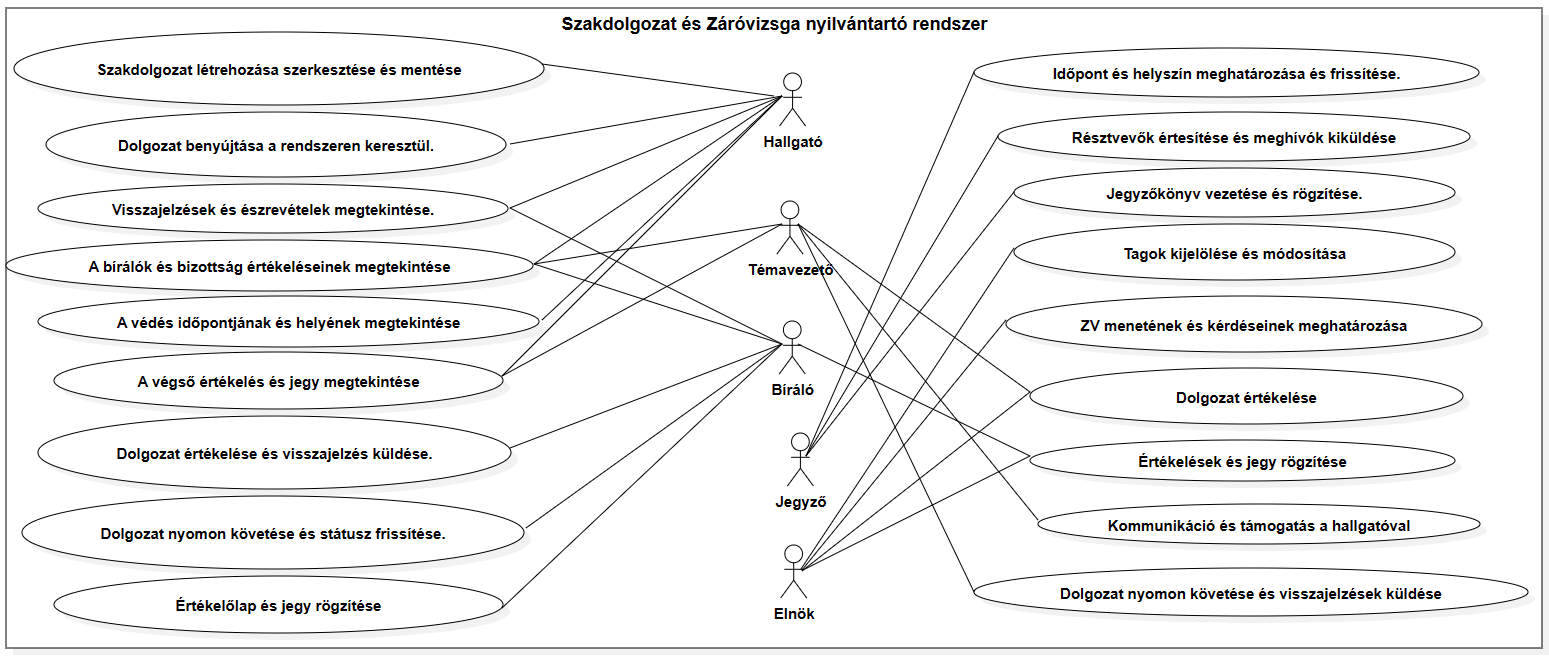
\includegraphics[width=\textwidth]{images/UseCaseDiagram1.pdf}
\caption{Az alkalmazás use case diagramja}
\label{fig:usecase}
\end{figure}
\newpage

\Section{Folyamatok ábrázolása}

Az alkalmazás tervezésekor több folyamatot is figyelembe kellett vennem, mint például a bírálati folyamatot és a bírálat feltöltésének lépéseit. Ezeket a folyamatokat szekvenciadiagramon és folyamatábrán ábrázoltam.

\subsection{Bírálati folyamat}

\vspace{0.5cm}

\begin{enumerate}
\item \textbf{Adminisztrátor regisztrálja a hallgatót:}

Az adminisztrátor bejelentkezik az alkalmazásba és regisztrálja a hallgatót a rendszerbe.
A regisztráció során az adminisztrátor rögzíti a hallgató nevét, e-mail címét, jelszavát és egyéb szükséges információkat.

\item \textbf{Témavezető értesíti az adminisztrátort a bíráló elérhetőségéről:}

A témavezető értesíti az adminisztrátort arról, hogy mely bírálók érhetők el a szakdolgozat bírálásához. 

\item \textbf{Adminisztrátor regisztrálja a bírálót:}

Az adminisztrátor rögzíti a bíráló adatait az alkalmazásban, beleértve a nevet, e-mail címet, jelszót és egyéb szükséges információkat. A regisztráció után a bíráló jogosult lesz részt venni a bírálati folyamatban.

\item \textbf{Elnök felkéri a témavezetőt és a bírálót a bírálatra:}

Az elnök bejelentkezik az alkalmazásba és kiválasztja a szakdolgozatot, amelyre bírálatot kíván kérni. Az elnök elküldi a felkérést a bírálat elvégzésére a témavezetőnek, és a kiválasztott bírálónak.

\item \textbf{Bíráló és a témavezető elkészíti a bírálatot:}

A bíráló és a témavezető bejelentkezik az alkalmazásba, ahol elérhetik a kijelölt szakdolgozatot. A bíráló és a témavezető részletesen értékeli a dolgozatot, és dokumentálja az észrevételeit.

\item \textbf{Elnök kiküldi a bírálatot a hallgatónak:}

Az elnök bejelentkezik a platformra, ahol hozzáfér a bírálati eredményekhez.
Az elnök elküldi a bírálati eredményeket a hallgatónak, lehetővé téve számára azok megtekintését.
\end{enumerate}

\newpage

\begin{figure}[h]
\centering
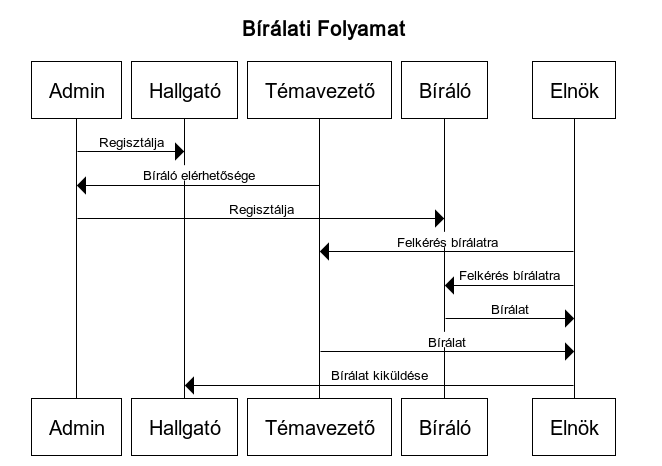
\includegraphics[scale=0.8]{images/Bírálati_folyamat.png}
\caption{Bírálati folyamat szekvenciadiagramja}
\label{fig:biralati_folyamat}
\end{figure}

\subsection{Bírálat feltöltésének lépései}

\begin{enumerate}

\item \textbf{Bíráló belép a rendszerbe és listázza a felkéréseket:}

A bíráló bejelentkezik az alkalmazásba. Miután sikeresen bejelentkezett, a rendszer megjeleníti a bíráló számára elérhető felkéréseket. A felkérések listája tartalmazza az összes olyan szakdolgozatot, amelyekre a bírálót felkérték a bírálat készítésére.

\item \textbf{Bíráló kiválaszt egy felkérést a listából:}

A bíráló kiválasztja a listából azt a szakdolgozatot, amelyre bírálatot szeretne készíteni.

\item \textbf{Bíráló elkezdi szerkeszteni a bírálatot:}

Elkezdi szerkeszteni a bírálatot. Részletesen értékeli a dolgozatot és dokumentálja az észrevételeit, pontozását vagy egyéb megjegyzéseit a bírálatban.

\item \textbf{Bíráló beküldi a szerkesztett bírálatot:}

Miután a bíráló elkészítette a bírálatot, beküldi azt a rendszerbe.

\item \textbf{Ellenőrzés:}

A rendszer ellenőrzi a beküldött bírálatot, hogy megfelel-e a formai követelményeknek.
\begin{itemize}
\item Ha a bírálat formailag nem megfelelő:
A rendszer hibaüzenetet jelenít meg, és figyelmezteti a bírálót a hibákra.
A bíráló visszairányításra kerül a bírálat szerkesztéséhez, hogy kijavítsa a hibákat.
\item Ha a bírálat megfelelő formában van beküldve:
A rendszer értesítést küld a bírálónak a sikeres beküldésről, illetve a dokumentum azonnal letöltődik, amit meg tud tekinteni.
\end{itemize}

\item \textbf{Sikeres beküldés:}

Miután a bíráló sikeresen ellenőrizte és beküldte a bírálatot, a folyamat befejeződik, és a bíráló visszatér az alkalmazás főoldalára vagy más tevékenységekhez.

\end{enumerate}

\begin{figure}[h]
\centering
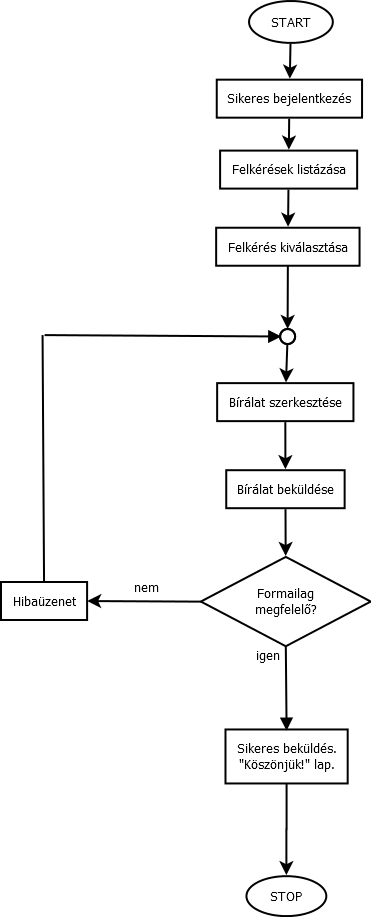
\includegraphics[scale=0.5]{images/Bírálat_feltöltése.png}
\caption{Bírálati feltöltéseinek lépései}
\label{fig:birala_feltoltese}
\end{figure}

\newpage

\Section{Lapok közötti átmenetek}

Az alábbi ábrák és a leírások különböző szerepkörök nézőpontjából ábrázolják, hogy melyik oldalhoz férhetnek hozzá. Fontos megjegyeznem, hogy nincs összeköttetés az angular komponensek és a 3.fejezet elnevezései között.

\subsection{Elnök és Jegyző}

\begin{figure}[h]
\centering
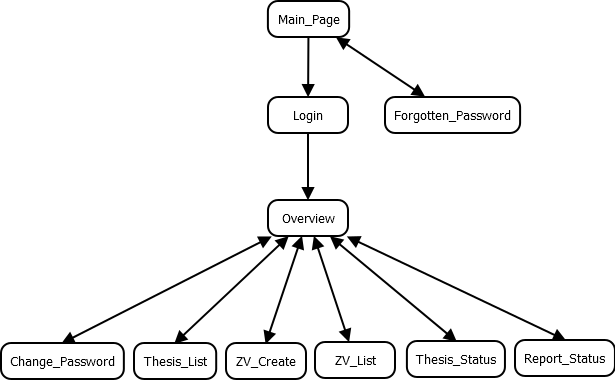
\includegraphics[scale=0.5]{images/Elnok.png}
\caption{A webalkalmazás az elnök szemszögéből}
\label{fig:elnok}
\end{figure}

\begin{itemize}

\item \textbf{Bejelentkezés:} Minden felhasználó lehetőséget kap a belépésre az alkalmazásba, ahhoz hogy azonosíthassák magukat és hozzáférjenek a rendszerhez. Ehhez felhasználónevet és jelszót kell megadniuk.

\item \textbf{Elfelejtett jelszó:} Ha a felhasználók elfelejtik a jelszót, lehetőségük van új igénylésére. Erre az Elfelejtett jelszó menüpont szolgál, amely segítségével új jelszó kérése vagy generálása lehetséges.

\item \textbf{Jelszó változtatás:}Az alkalmazás felhasználói képesek megváltoztatni jelszavukat, ha szükségük van rá. Erre a Jelszó változtatás lap szolgál, ahol lehetőség van a jelszó módosítására.

\item \textbf{Szakdolgozatok listázása:} Az elnök és a jegyző is képes kilistázni a rendszerben található összes szakdolgozatot. Ez lehetőséget ad arra, hogy áttekintsék a szakdolgozatok részleteit.

\item \textbf{Záróvizsgák létrehozása és listázása:} Mindkét szerepkörnek lehetősége van létrehozni és kilistáztatni záróvizsgákat a platformon.

\item \textbf{Szakdolgozatok státusza:} Az elnök és a jegyző képes megtekinteni a szakdolgozatok aktuális státuszát az alkalmazásban. Ez lehetőséget ad számukra, hogy nyomon kövessék a dolgozatok előrehaladást.

\item \textbf{Bírálat státusza:} Az elnök és a jegyző bírálókat tud felkérni a szakdolgozatok értékelésére, valamint nyomon tudják követni a bírálati folyamatot. Ezenkívül lehetőségük van letölteni a bírálatokat és e-mailben elküldeni a hallgatóknak.

\item \textbf{Záróvizsga jegyzőkönyv generálása} (jegyző számára): A jegyző külön lehetőséget kap arra, hogy generáljon záróvizsga jegyzőkönyveket az alkalmazásban, ami segíti az adminisztrációt és a dokumentációt a záróvizsgákhoz kapcsolódóan.
\end{itemize}



\subsection{Bíráló és Témavezető}

\begin{figure}[h]
\centering
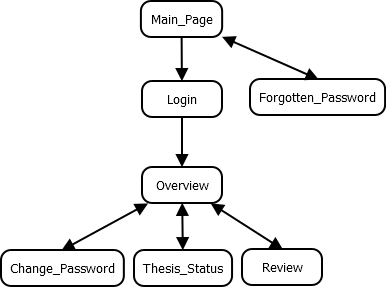
\includegraphics[scale=0.5]{images/Biralo.png}
\caption{A webalkalmazás a bíráló és témavezető szemszögéből}
\label{fig:biralo_temavezeto}
\end{figure}

\begin{itemize}

\item \textbf{Bírálat írása:} A témavezető és a bíráló bírálatokat tud írni a szakdolgozatokról. Fontos megjegyezni, hogy csak azokra a dolgozatokra tudnak bírálatot írni, amelyekre fel lettek kérve. A bírálatok általában értékelést és észrevételeket tartalmaznak a dolgozat tartalmával kapcsolatban.

\item \textbf{Szakdolgozatok státusza:} Mindkét felhasználó képes megtekinteni azokat a szakdolgozatokat, amelyekre fel lettek felkérve. Ez lehetőséget ad számukra, hogy letölthessék és megtekintsék a dolgozatokat.

\end{itemize}

\subsection{Hallgató}

\begin{figure}[h]
\centering
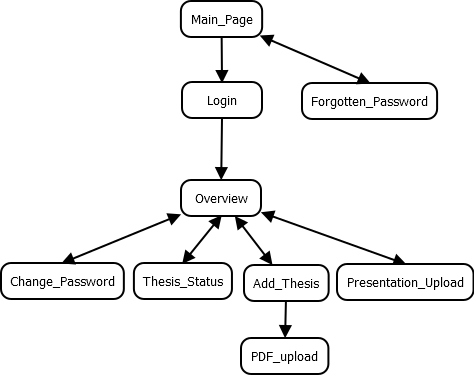
\includegraphics[scale=0.5]{images/Hallgato.png}
\caption{A webalkalmazás a hallgató szemszögéből}
\label{fig:hallgato}
\end{figure}

\begin{itemize}

\item \textbf{Szakdolgozat adatainak kitöltése:} A hallgatónak a feltöltött szakdolgozathoz kapcsolódó adatokat kell megadnia, például a dolgozat címét, szerzőjét, konzulensét stb. Ez lehetőséget ad az adminisztrátornak és a többi felhasználónak a dolgozat könnyebb azonosítására és kezelésére.

\item \textbf{Szakdolgozat feltöltése:} A hallgatónak lehetősége van a szakdolgozatát feltölteni az alkalmazásba. A szakdolgozat adatainak kitöltése után a rendszer átnavigálja a hallgatót erre a felületre, ahol feltöltheti a szakdolgozat dokumentumát és a csatolmányt.

\item \textbf{Szakdolgozat státusza:} A hallgatónak lehetősége van megtekinteni a feltöltött szakdolgozatának aktuális státuszát az alkalmazásban. 

\item \textbf{Prezentáció feltöltése:} Ez egy olyan funkció, ami lehetőséget biztosít a hallgatónak arra, hogy a szakdolgozatának megvédéséhez szükséges prezentációt is feltölthesse az alkalmazásba.


\end{itemize}


\subsection{Adminisztrátor}

Az adminisztrátor szerepe az alkalmazásban a legteljesebb hozzáférést biztosítja az összes funkcionalitáshoz, valamint az alábbi plusz feladatokat látja el:

\begin{itemize}

\item \textbf{Felhasználók felvitele:} Az adminisztrátornak lehetősége nyílik új felhasználókat regisztrációjára.

\item \textbf{Felhasználók listázása és kezelése:} Az admin képes kilistázni az összes felhasználót az alkalmazásban. Lehetősége van az adatokat megtekinteni, módosítani és törölni.

\end{itemize}
